\chapter{Tiny trainable instruments}

\epigraph{All the modern things \\ have always existed \\ they've just been waiting}{The Modern Things \\ Björk, 1995}

This chapter describes the process of conceptualizing and developing this thesis project, which is an antidisciplinary project, drawing from the disciplines of \acrshort{AI}, electrical engineering, computer science, media arts, music, and pedagogy, among others.

First there is a definition of the words that make up the title of this project, and then an overview and explanation of the main components of this thesis , which include:

\begin{enumerate}
  \item TinyTrainable Arduino software library
  \item Auxiliary code for \acrshort{ML}
  \item Workshop educational material
\end{enumerate}

\section{Definition of Tiny trainable instruments}

\subsection{Definition of tiny}

Bi tiny I mean handheld, lightweight instruments that you can take for a walk or on your backpack. Tiny is also a nod to the new uprising field of tiny \acrshort{ML}.

\subsection{Definition of trainable}

By trainable I mean a computational device that can learn by examples. This name comes from the \acrshort{ML} lexicon, where training is a process where an algorithm finds the numerical values of all parameters (weights, biases) of a \acrshort{ML} model, with the help of a dataset.

The process of training a model with a microcontroller has been really rewarding for me during the making of this thesis. When I program audiovisual computational devices to react to sensors, I often find myself having to look at streams of data, having to program statistical methods to detect trends, such as averages, and then having to program a hard coded value on the software, and having to write a manual for setup or fine tuning for collaborators to be able to run it again under different conditions.

The fact that I can program once, and then train on device, with the algorithm taking care of finding correlations, make for a more flexible workflow that I am hoping can be included in the toolkit of artists.

\subsection{Definition of instruments}

By instruments I mean devices that act as transducers across mediums, processing an input, which results in an output.

 A musical example is the guitar, where the input strumming results in output sound. I mention the guitar because of its nonlinear and flexible behavior, with multiple different ways of strumming, even by non-human agents, resulting in infinite sounds.

Another of my favorite instruments is the bicycle, which I like to define as a device that converts the input pedalling into all sorts of outputs: adventure, sweat, and wind in your face.

\section{Dreams and goals}

We are surrounded by devices that are listening us.

TODO: insert picture of surveillance camera near my home, in the middle of nature.

I not only have algorithms

TODO: insert picture of garbled zoom speech to text, failing with my speech.

Dream: drum machine i can talk to, like The White Stripes also perform changes in realtime midset with no playlist.  



The Tiny trainable instruments 

\begin{table}[ht]
    \centering
    \begin{tabular}{ | l | l | l | l | l | l | l | l |}
        \hline
        \textbf{\backslashbox{Input}{Output}}  & Buzzer & LED & \acrshort{MIDI} & Printer & Screen & Serial & Servo \\
        \hline
        Color & & & & & & & \\
        \hline
        Gesture & & & & & & & \\
        \hline
        Speech & & & & & & & \\
        \hline
    \end{tabular}
    \caption{Matrix of inputs and outputs}
    \label{table:tiny-trainable-instruments-inputs-outputs-matrix}
\end{table}{}

\begin{table}[ht]
    \centering
    \begin{tabular}{ | l | l | l |}
        \hline
        \textbf{Input}  & \textbf{Sensor library} & \textbf{\acrshort{ML} library} \\
        \hline
        Color &  Arduino{\_}APDS9960 & Arduino{\_}KNN \\
        \hline
        Gesture & Arduino{\_}LSM9DS1 & Arduino{\_}TensorFlowLite \\
        \hline
        Speech & PDM & Arduino{\_}TensorFlowLite \\
        \hline
    \end{tabular}
    \caption{Software dependencies for inputs}
    \label{table:software-dependencies-inputs}
\end{table}{}

\begin{table}[ht]
    \centering
    \begin{tabular}{ | l | l | }
        \hline
        \textbf{Output}  & \textbf{Actuator library} \\
        \hline
        Buzzer & - \\
        \hline
        LED & - \\
        \hline
        \acrshort{MIDI} & - \\
        \hline
        Printer & Adafruit Thermal Printer Library\\
        \hline
        Screen & Adafruit{\_}SSD1306\\ 
        \hline
        Serial & - \\
        \hline
        Servo & Servo\\
        \hline
    \end{tabular}
    \caption{Software dependencies for outputs}
    \label{software-dependencies-outputs}
\end{table}{}

\begin{figure}[ht]
  \centering
  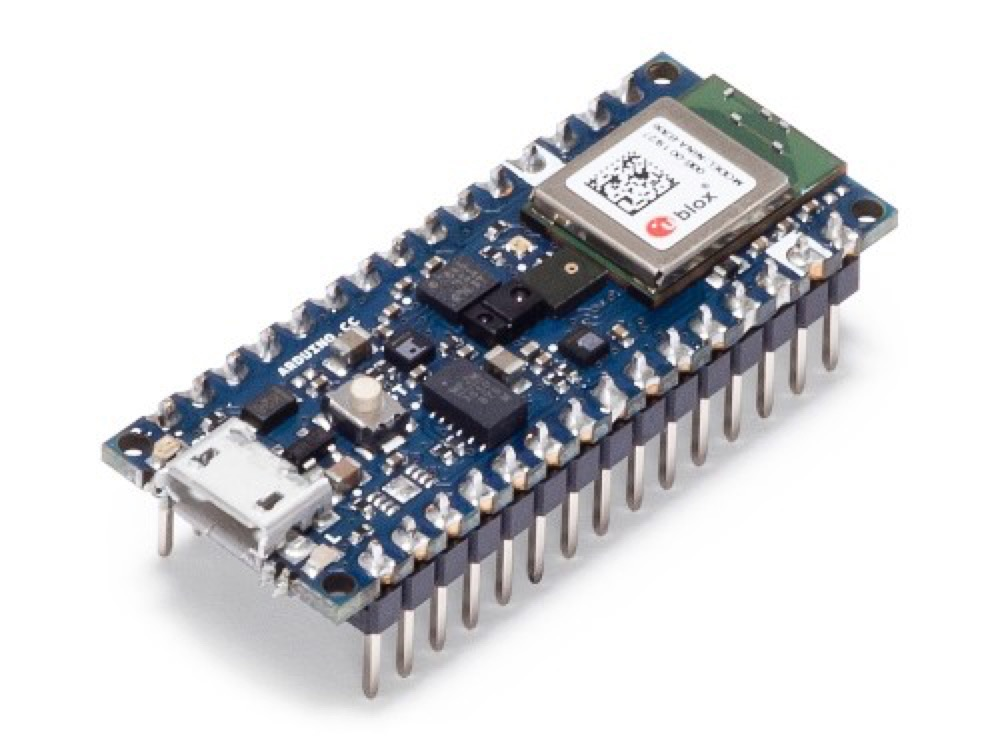
\includegraphics[width=0.75\linewidth,height=0.25\textheight,keepaspectratio]{images/materials-arduino-nano-33-ble-sense.jpg}
  \caption{Arduino Nano 33 BLE Sense microcontroller with headers}
  \caption*{Retrieved from \cite{website-materials-arduino-nano-33-ble-sense}}
  \label{fig:materials-arduino-nano-33-ble-sense}
\end{figure}

\section{TinyTrainable Arduino software library}

The main contribution of this thesis is the TinyTrainable Arduino library, an open source library for creating Tiny Trainable instruments, as in microcontroller-based devices that you can train to react to gestures with \acrshort{ML}, so they can process and output different multimedia events, such as sound, movement, light, and text.
s
\subsection{Repository structure}

The library is a repository hosted at \url{https://github.com/montoyamoraga/TinyTrainable}, where you can review all the history and commits through time, to see how the library or each file has evolved over time.

The structure of the folders follows 2 simultaneous specifications: it includes the necessary file and folder names for being packaged and indexed as an Arduino Library, and also it complies with GitHub guidelines for licensing and automatic workflows for testing the code.

The source code of the library is written in C++ and is located in the src/ folder. The examples live in the examples/ folder, and are written in Arduino. Some trained \acrshort{ML} models are included as C++ files on the assets/ folder.

\subsection{Installation}

The library can be downloaded from the Releases section of the repository at  \url{https://github.com/montoyamoraga/TinyTrainable/releases}, where you also have access to the complete history of releases over time. To install it, you need to uncompress the .zip into a folder, and then make it discoverable by the Arduino IDE.

Since that method can be cumbersome and prone to errors, I made the effort to publish the TinyTrainable library, by complying with the latest Arduino Library Manager specifications, detailed on their repository \url{https://github.com/arduino/library-registry/}. With that, from the Arduino IDE you can open their Library Manager and do a one-click installation of the library, or even with the Arduino CLI you can install it via the command line on your machine.

\subsection{Hardware basics}

This library has only 1 fixed hardware requirement: it only runs on the Arduino Nano 33 BLE Sense, a microcontroller released in 2019. This library relies on the microcontroller's embedded sensors, so there is no need for wiring extra components.

For power you need a generic micro USB cable to provide the necessary input of 5V to the Arduino microcontroller. To upload code to the microcontroller you can use the same USB cable to connect to a computer running the Arduino IDE.

\begin{figure}[ht]
  \centering
  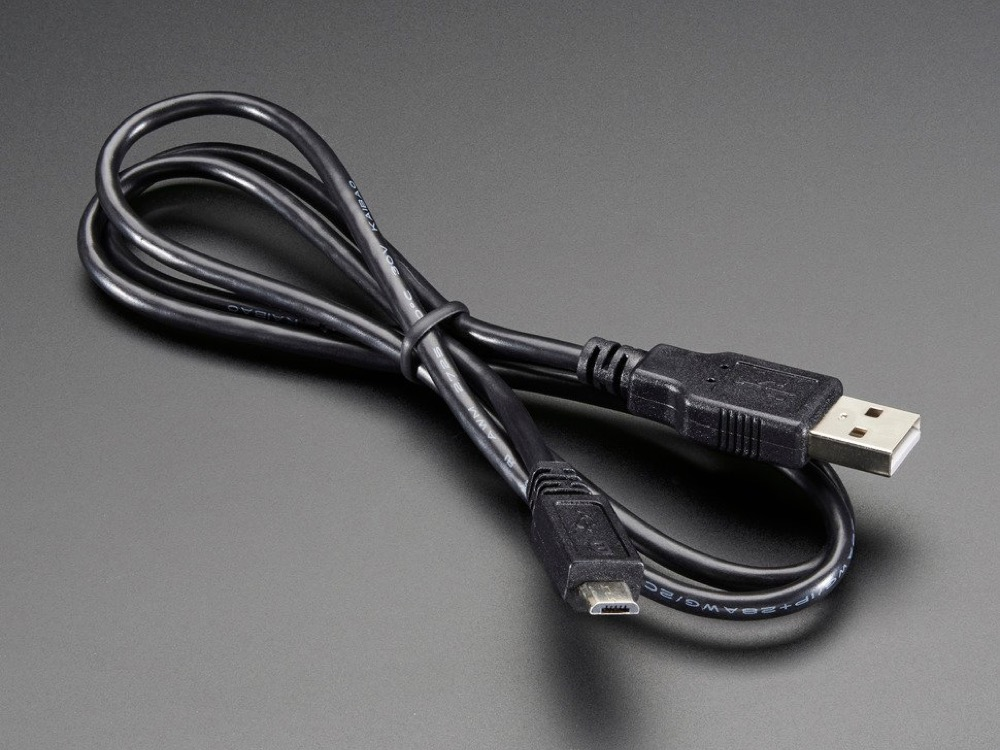
\includegraphics[width=0.75\linewidth,height=0.25\textheight,keepaspectratio]{images/materials-adafruit-micro-usb-cable.jpg}
  \caption{Micro USB cable}
  \caption*{Retrieved from \cite{website-materials-adafruit-micro-usb-cable}}
  \label{fig:materials-adafruit-usb-cable}
\end{figure}

To build your instrument, you need a breadboard, jumper wires, and one of the many possible output devices that we describe in the following section.

\begin{figure}[ht]
  \centering
  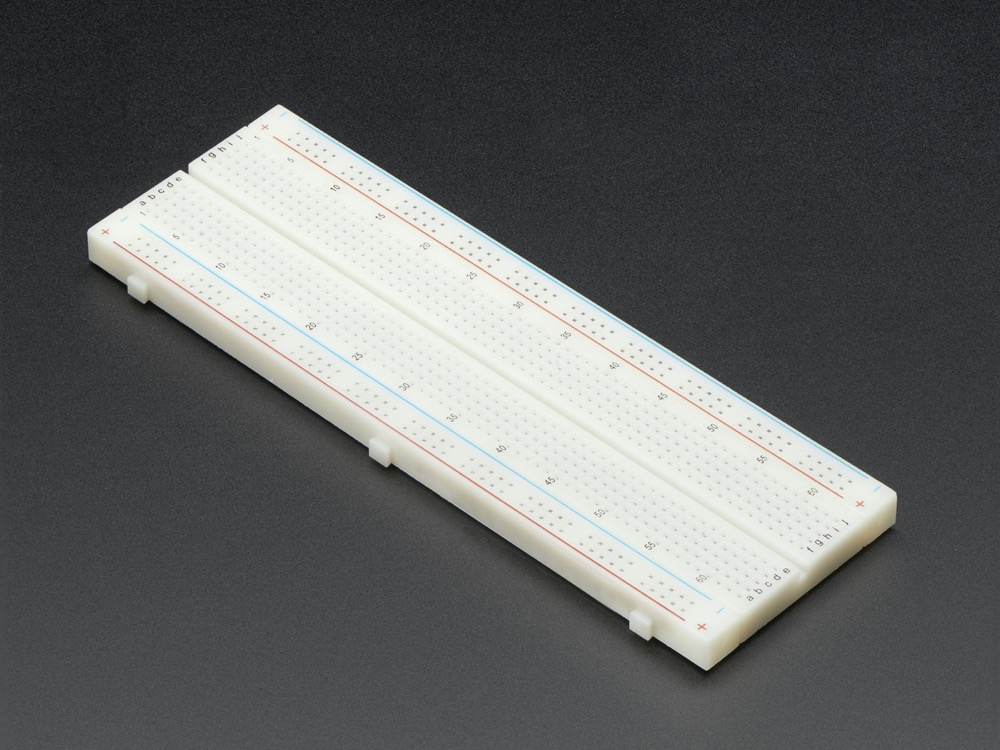
\includegraphics[width=0.75\linewidth,height=0.25\textheight,keepaspectratio]{images/materials-adafruit-breadboard.jpg}
  \caption{Breadboard}
  \caption*{Retrieved from \cite{website-materials-adafruit-breadboard}}
  \label{fig:materials-adafruit-breadboard}
\end{figure}

\begin{figure}[ht]
  \centering
  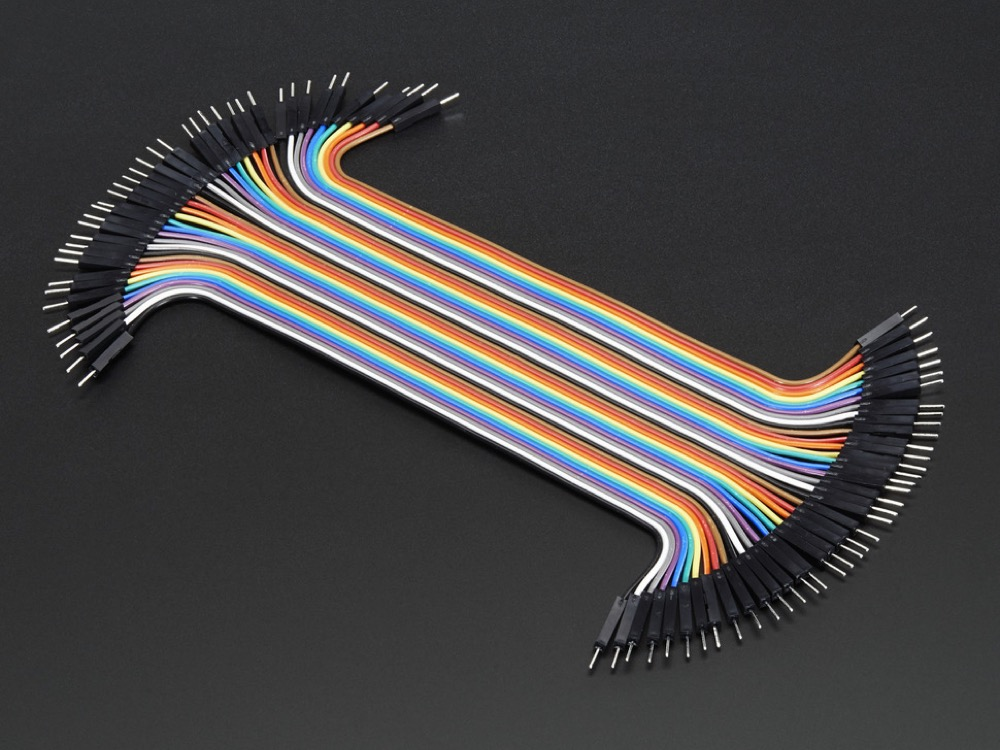
\includegraphics[width=0.75\linewidth,height=0.25\textheight,keepaspectratio]{images/materials-adafruit-jumper-wires.jpg}
  \caption{Jumper wires}
  \caption*{Retrieved from \cite{website-materials-adafruit-jumper-wires}}
  \label{fig:materials-adafruit-jumper-wires}
\end{figure}

\subsection{Hardware for outputs}

The TinyTrainable library supports a 

UNTILHERE

\section{Technology stack}

This project is built with microcontrollers and 

\section{Design principles}

This thesis tries to 

\begin{enumerate}
  \item Affordable
  \item Hackable
  \item Open
  \item Private
\end{enumerate}

\subsection{Cheap}

The materials for this thesis 


\section{Open}

All examples included with this library were written with the aim of showing the fundamentals of how to build the instruments and different \acrshort{ML} enabled manipulation of multimedia material, so that people could build on top of it and make it their own, by changing the values of variables and adding more functionalities.

\section{Philosophy and experience}

Throughout this project, the magic number was 3. The \acrshort{ML} algorithms were hardcoded to be able to distinguish between 3 different categories: 3 colors, 3 physical gestures, 3 sound utterances.

\section{Inputs}

We are using the RGB color, proximity, gyroscope, accelerometer, and microphone sensors on the microcontroller, in order to capture the Inputs

\begin{enumerate}
  \item Color
  \item Gesture
  \item Speech
\end{enumerate}

\subsection{Color}

This approach uses the RGB color sensor from the microcontroller, with the auxiliary help from the proximity sensor, that is used to capture color information at a certain distance threshold.

The data is passed to a k-Nearest-Neighbor algorithm, programmed using the Arduino KNN library.

\subsection{Gesture}

This input uses the information from the Inertial Measurement Unit (IMU) of the microcontroller, including a gyroscope and accelerometer. It captures data after a certain threshold of movement is detected.

The data is passed to a TensorFlow neural network, programmed using the Arduino TensorFlow Lite library, and based on the included magic$\_$wand example.

\subsection{Speech}

This input uses the information from the microphone of the microcontroller.

The data is passed to a TensorFlow neural network, programmed using the Arduino TensorFlow Lite library, and based on the included micro$\_$speech example.

\section{Outputs}

The different outputs were picked, because of their low cost, ubiquity, and possibilities of expansion and combining them.

\subsection{Buzzer}

This output creates pitched sound, by using a PWM output.

\begin{figure}[ht]
  \centering
  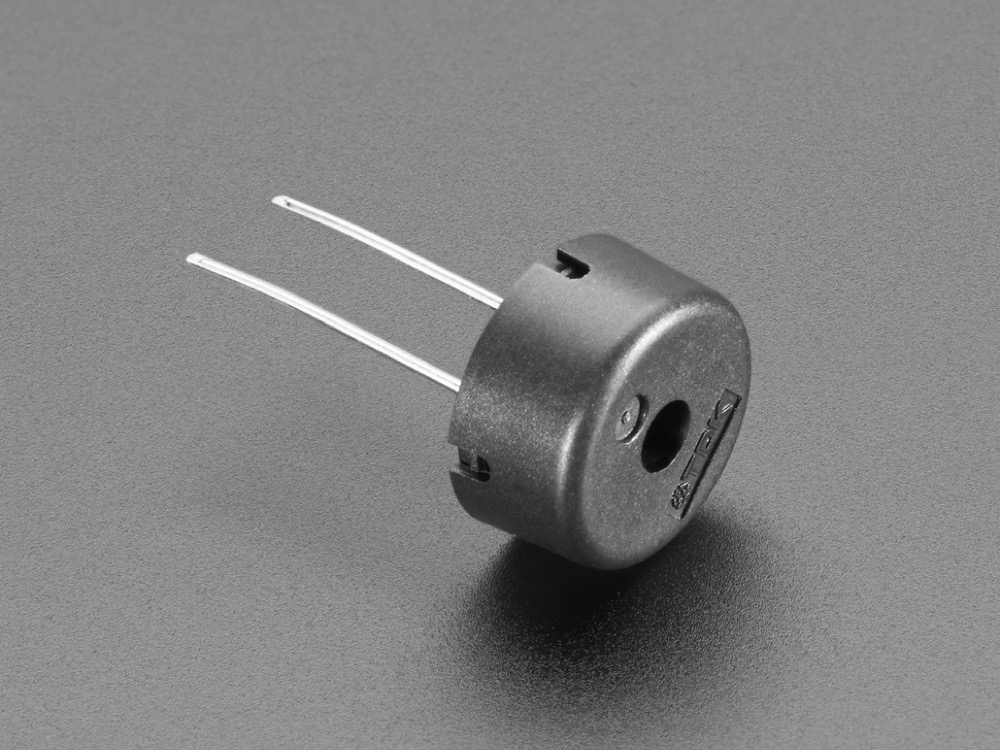
\includegraphics[width=0.75\linewidth,height=0.25\textheight,keepaspectratio]{images/materials-adafruit-buzzer.jpg}
  \caption{Buzzer}
  \caption*{Retrieved from \cite{website-materials-adafruit-buzzer}}
  \label{fig:materials-adafruit-buzzer}
\end{figure}

\subsection{LED}

This section requires no dependencies.

\begin{figure}[ht]
  \centering
  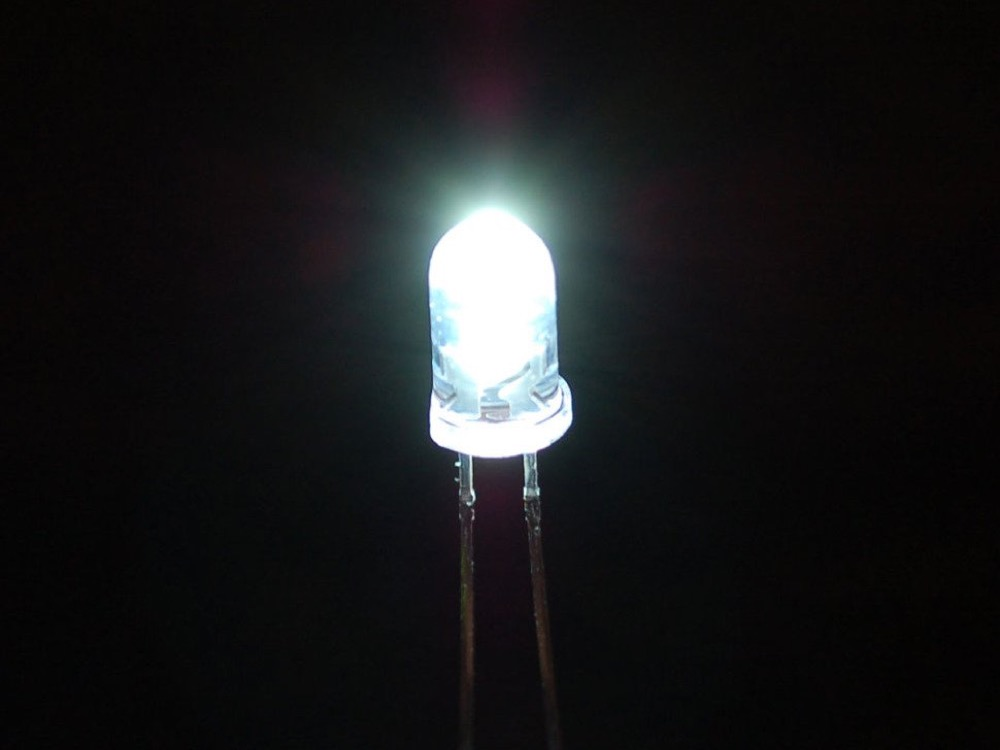
\includegraphics[width=0.75\linewidth,height=0.25\textheight,keepaspectratio]{images/materials-adafruit-led.jpg}
  \caption{LED}
  \caption*{Retrieved from \cite{website-materials-adafruit-led}}
  \label{fig:materials-adafruit-led}
\end{figure}

\subsection{MIDI}

We wrote functionalities to manipulate \acrshort{MIDI} instruments, and included examples to interface with some popular and cheap \acrshort{MIDI} instruments, such as the Korg volca beats.

We included examples for rhythmic and melodic elements, using two very ubiquitous and inexpensive \acrshort{MIDI} musical instruments, which are the Korg volca beats, and the Korg volca keys.

\begin{figure}[ht]
  \centering
  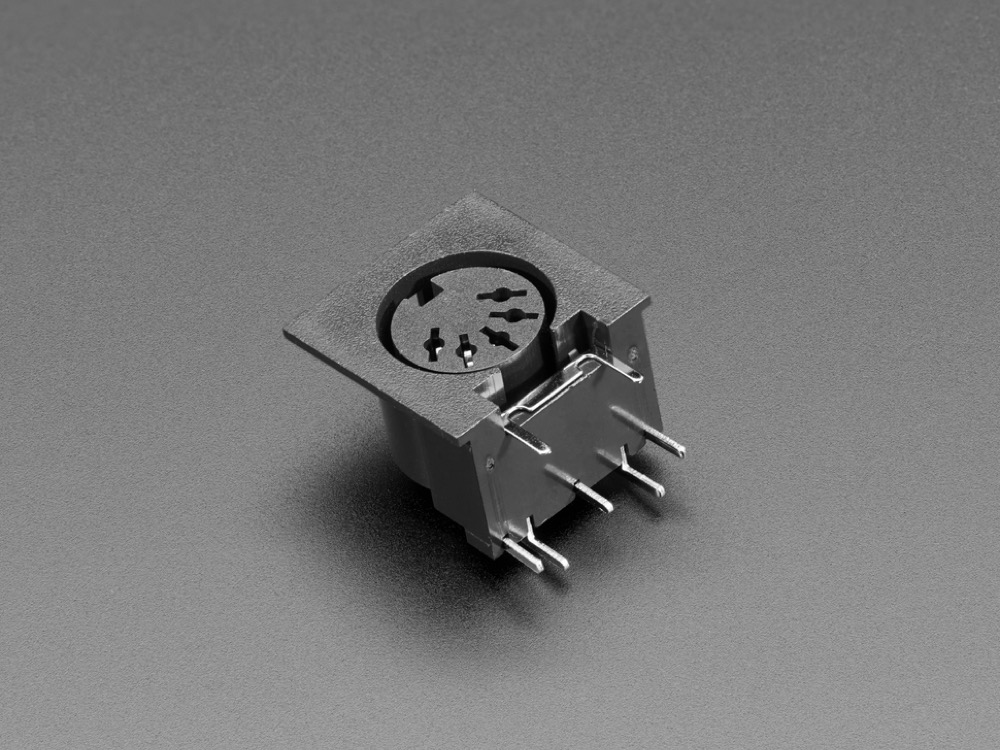
\includegraphics[width=0.75\linewidth,height=0.25\textheight,keepaspectratio]{images/materials-adafruit-midi-jack.jpg}
  \caption{MIDI jack}
  \caption*{Retrieved from \cite{website-materials-adafruit-midi-jack}}
  \label{fig:materials-adafruit-midi-jack}
\end{figure}

\subsection{Serial}

This output requires no library dependencies.

We use the already mentioned USB cable to connect to our computer, and receive messages over the serial port, available through the Arduino IDE.

\subsection{Screen}

This output requires a library for printing messages on a screen.

\begin{figure}[ht]
  \centering
  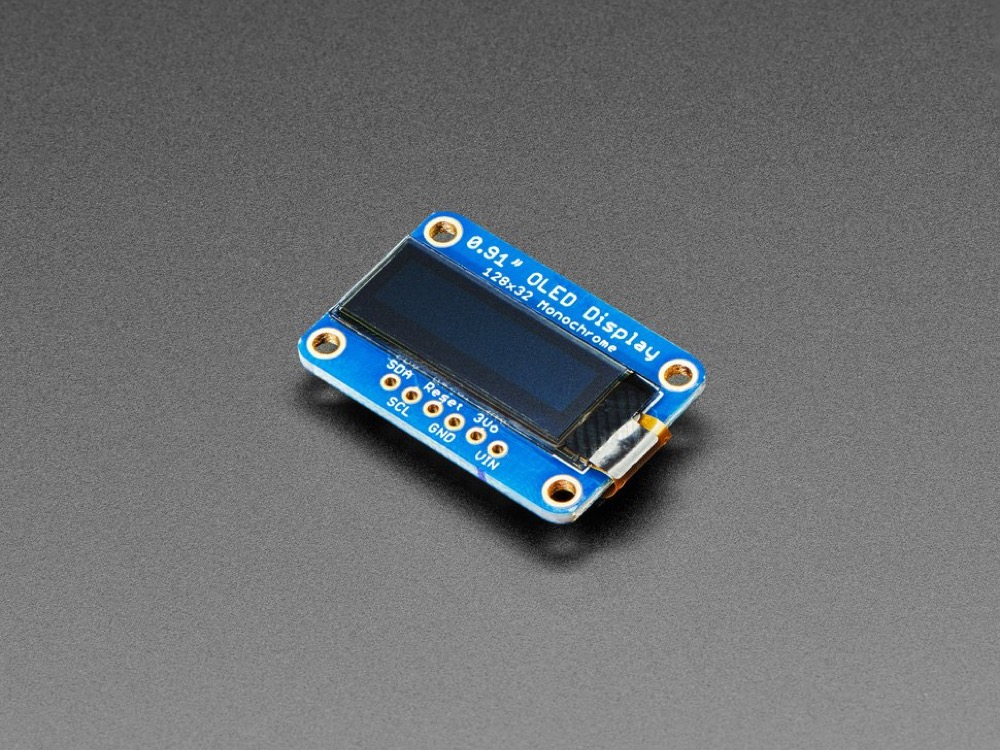
\includegraphics[width=0.75\linewidth,height=0.25\textheight,keepaspectratio]{images/materials-adafruit-screen.jpg}
  \caption{Screen}
  \caption*{Retrieved from \cite{website-materials-adafruit-screen}}
  \label{fig:materials-adafruit-screen}
\end{figure}

\subsection{Servo motor}

This output creates movement and through that, rhythmic sounds.

The main inspiration for this output was the emerging use of motor-activated percussive instruments, such as the Polyend Perc.

\begin{figure}[ht]
  \centering
  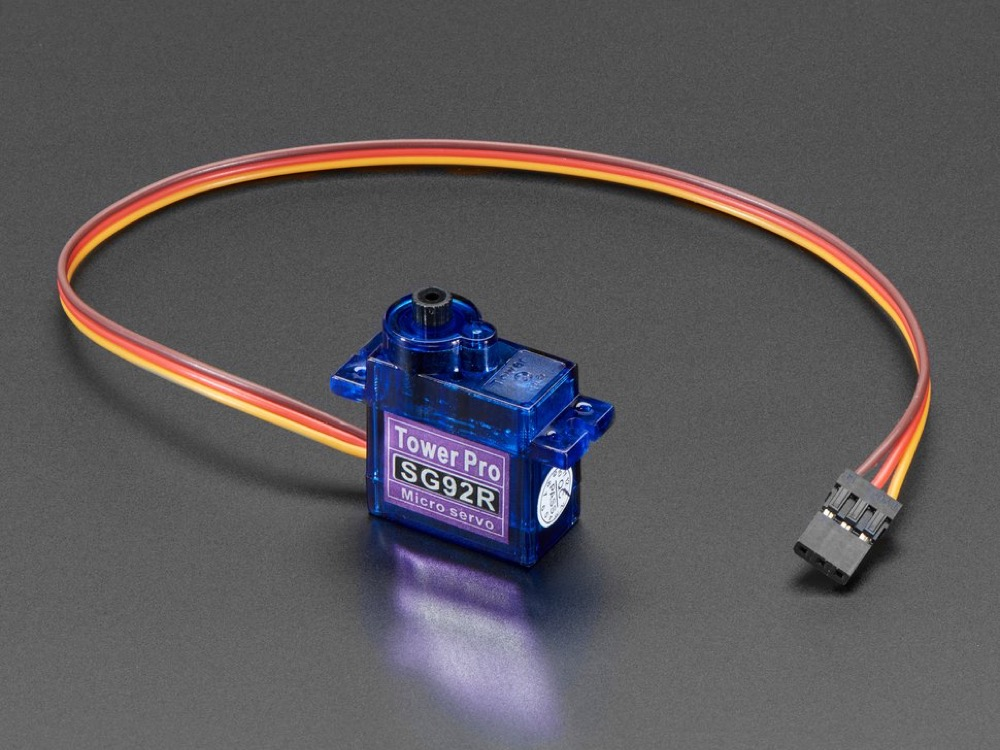
\includegraphics[width=0.75\linewidth,height=0.25\textheight,keepaspectratio]{images/materials-adafruit-servo.jpg}
  \caption{Micro servo motor}
  \caption*{Retrieved from \cite{website-materials-adafruit-servo}}
  \label{fig:materials-adafruit-servo}
\end{figure}

\subsection{Thermal printer}

A thermal printer is the basis for creating written and literary output, inspired by the field of computational poetry.

I used the popular Adafruit Thermal printer kit, which is documented on their website and includes a software library, distributed over GitHub and Arduino IDE, and also as a submodule on this project's TinyTrainable software library.

\begin{figure}[ht]
  \centering
  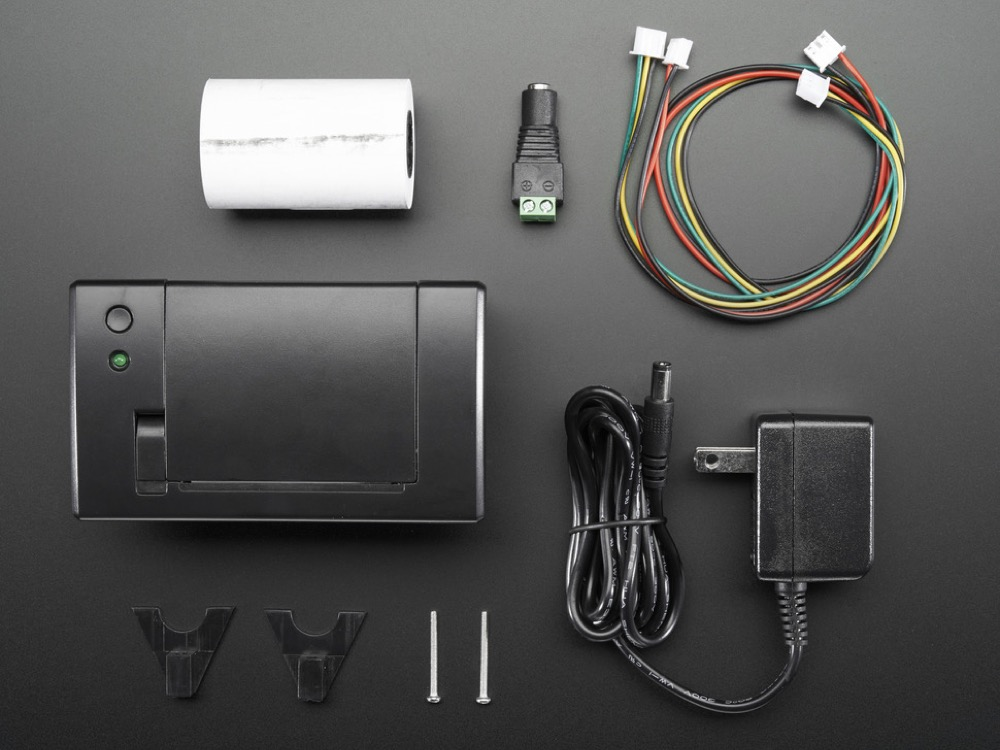
\includegraphics[width=0.75\linewidth,height=0.25\textheight,keepaspectratio]{images/materials-adafruit-thermal-printer.jpg}
  \caption{Thermal printer kit}
  \caption*{Retrieved from \cite{website-materials-adafruit-thermal-printer}}
  \label{fig:materials-adafruit-thermal-printer}
\end{figure}

\section{Development}

This thesis has been developed with the invaluable help of undergrad researchers Peter Tone and Maxwell Wang.

They have cloned both repositories, the main one and the Arduino library one, and have continuously submitted pull requests with their contributions.

Peter Tone has helped with research in data structures, library writing, and we have shared back and forth code, going from experimental proofs of concepts, and has also helped with the design of the user-facing library.

Maxwell Wang has proofread the code, has run the examples, and has helped with the writing of the documentation for self-learners and for the workshops.

We all share a Google Drive folder, where we all share notes about our research and development of the library and the educational material.

\section{Code}

This thesis is distributed as a repository, hosted on the GitHub platform, and available at https://github.com/montoyamoraga/tiny-trainable-instruments.

The auxiliary files, such as the LaTeX project for this document, and the auxiliary Jupyter notebooks, and documentation and tutorials are included on this repository.

The main software component of this project is the TinyTrainable library, available at https://github.com/montoyamoraga/TinyTrainable and also through the Arduino IDE.

The code included on this library is distributed on the folders:

\begin{enumerate}
  \item examples/
  \item src/
\end{enumerate}

\subsection{src/}

The source code for where there is a TinyTrainable.h and TinyTrainable.cpp file where we included all the basic functionality of the library. Additional subfolders include

\subsubsection{inputs/}

Base class Input and inherited classes for each one of the other inputs.

\subsubsection{outputs/}

Base class Output and inherited classes for each one of the other outputs.

\subsubsection{tensorflow/}

Auxiliary files, copied from the examples from the Arduino TensorFlow Lite that we are building on top of, and also from the newer TinyML library by the EdX team. These, unless otherwise noted, are included without modifications and distributed through the Apache License included on each file's headers.

\section{Tools}

This is a summary of tools used for making this project.

\subsection{clang-format}

Tool for automation of formatting to source code. More information at \url{https://clang.llvm.org/docs/.ClangFormat.html}.

\section{Doxygen}

Tool for generating documentation from the source code. More information at \url{https://www.doxygen.nl/}.

\subsection{GitHub Actions}

Every time we push code to the TinyTrainable repositories, a GitHub action creates a virtual machine, and runs a script to generate the Doxygen documentation and push it to the gh-pages branch, hosted at \url{https://montoyamoraga.github.io/TinyTrainable}.

\subsection{Jupyter}

Jupyter is a free, open-source browser application that allows users to easily read and write code in a clean, accessible environment. Code is segmented into cells, which users can execute individually by clicking into and selecting the triangle "play" button at the top. Subsequent code executes based on operations done in previous cells. Basically, Jupyter notebooks allow programmers to create clean, step-by-step interactive walkthroughs through their code. More information at \url{https://jupyter-notebook-beginner-guide.readthedocs.io/en/latest/index.html}.
\subsection{Markdown}

Markdown is a lightweight markup language with simple, intuitive syntax. Aside from a few key differences, it is largely the same as plaintext. The documentation of this project is written using Markdown, including this document! More info at \url{https://guides.github.com/features/mastering-markdown/}
